\documentclass[12pt,a4paper]{report}
\usepackage[utf8]{inputenc}				% Support de l'UTF-8
\usepackage[french]{babel} 				%
\usepackage[T1]{fontenc}				%
\usepackage{graphicx}					%
\usepackage[a4paper,					% Définit les marges
	headheight=45pt,headsep=35pt,		%
	left=1in,right=1in,					%
	top=1.6in,bottom=1.2in]{geometry}	%
\usepackage{lastpage} 					% Numérotation des pages
\usepackage{fancyhdr}					% Pour le header et le footer
\usepackage[normalem]{ulem}				% Soulignement
\usepackage{framed}						% Pour les tableaux des E/S
\usepackage{tcolorbox}			%
\usepackage{multicol}					% Gestion du nombre de colonnes
\usepackage{wrapfig}					%
\usepackage{caption}					% Centrage de la légende

% Justification du texte
\newcommand*\justify{		%
  \fontdimen2\font=0.4em	% interword space
  \fontdimen3\font=0.2em	% interword stretch
  \fontdimen4\font=0.1em	% interword shrink
  \fontdimen7\font=0.1em	% extra space
  \hyphenchar\font=`\-		% allowing hyphenation
}

% Infos du document
\author{INSAlgo}
\title{ShaKer 2019 PreCoding Battle - Problème A}

% En-tête et pied de page
\pagestyle{fancy}
\renewcommand{\headrulewidth}{0pt}				% Pas de bordure sous l'en-tête
\lhead{{\huge ShaKer 2019 PreCoding Battle}}		% En-tête gauche
\rhead{
\includegraphics[width=4cm]{logo.png}}	% En-tête droit
\rfoot{Page \thepage\,/\,\pageref{LastPage}}	% Pied de page droit
\cfoot{}										% Pied de page central

\begin{document}

\begin{center}
	{\Large A. « Sortie en bus »}
	\bigskip
\end{center}

\section*{Problème}

\begin{wrapfigure}{r}{0.5\textwidth}
    \centering
    \captionsetup{justification=centering}
    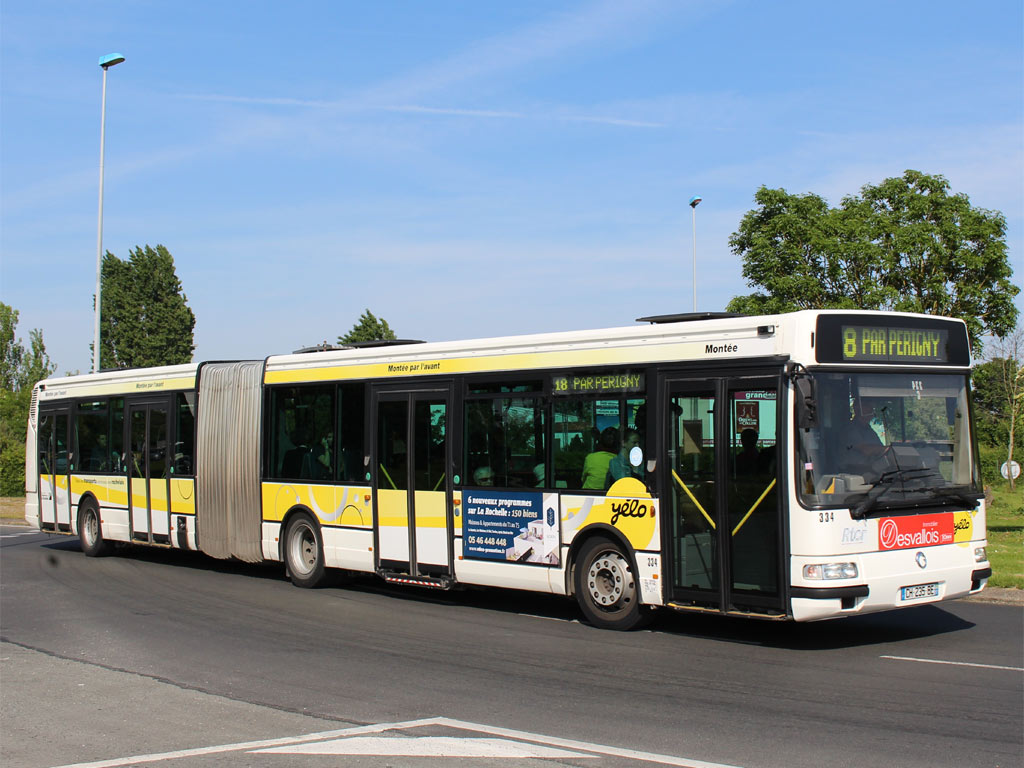
\includegraphics[width=0.45\textwidth]{bus.jpg}
    \caption*{Un bus de votre compagnie}
\end{wrapfigure}
Vous dirigez une compagnie nationale de transport de bus et vous êtes face à un gros problème technique: une maison de retraite souhaite faire une visite au musée, et ne sait pas combien de bus elle doit réserver. 

Vous allez donc écrire un programme permettant de résoudre ce problème en déterminant le nombre de bus nécessaires pour le transport de tous les passagers. \\


\subsection*{Entrée}%Section des INPUT
Sur 2 lignes~:
\begin{itemize}
\item un entier $N$ représentant le nombre de personnes souhaitant participer à la visite ($0 \leq N \leq 10^{4}$)~;
\item un entier $P$ représentant le nombre de places dans un bus ($1 \leq P \leq 10^{4}$).
\end{itemize}
\textit{Note~: Tous les bus ont le même nombre de places.}

\subsection*{Sortie}
\begin{itemize} %Section des OUTPUT
\item Afficher un entier (sur la sortie standard) correspondant au nombre de bus à réserver.
\end{itemize}

\section*{Exemple}%Section Exemple
\begin{minipage}{\linewidth}

%Pour un exemple copier d'ici à ...
\begin{multicols}{2}
	\begin{tcolorbox}[title=Entrée,width=\linewidth,arc=0mm,colbacktitle={white!80!black},coltitle=black]
		\begin{verbatim}
10
5
		\end{verbatim}
	\end{tcolorbox}
\columnbreak
	\begin{tcolorbox}[title=Sortie,width=\linewidth,arc=0mm,colbacktitle={white!80!black},coltitle=black]
		\begin{verbatim}
2
        \end{verbatim}
	\end{tcolorbox}
\end{multicols}
On a ici 10 personnes à transporter et 5 places par bus~; 2 bus sont donc suffisants.

%... à ici pour la fin d'un exemple. Penser à mettre plusieurs exemples

%Pour un exemple copier d'ici à ...
\begin{multicols}{2}
	\begin{tcolorbox}[title=Entrée,width=\linewidth,arc=0mm,colbacktitle={white!80!black},coltitle=black]
		\begin{verbatim}
17
7
		\end{verbatim}
	\end{tcolorbox}
\columnbreak
	\begin{tcolorbox}[title=Sortie,width=\linewidth,arc=0mm,colbacktitle={white!80!black},coltitle=black]
		\begin{verbatim}
3
        \end{verbatim}
	\end{tcolorbox}
\end{multicols}
On doit pouvoir transporter 17 personnes avec des bus de 7 places, il faut donc au minimum 3 bus (soit 21 places) pour y arriver.
%... à ici pour la fin d'un exemple. Penser à mettre plusieurs exemples

\end{minipage}

\bigskip



\end{document}